\chapter{Packing shapes on a Plane}

It is known that shape is an important attribute for crystal packings~\tocite, small changes in shape can lead to large changes in the packing fraction and the space group of the resulting crystal. The amorphous packing of shapes has not had the degree of study, focussing on ellipses and circles~\tocite. In this chapter I aim to elucidate the effects that shape has on amorphous packing and how they compare to the crystal packings. Along with generating this database of packing data I will also be looking to identify molecules that are resistant to crystal growth for further study in later chapters.

The two parameters of the Snowman molecule is the radius and the distance, searching the space of molecules can be done by sampling structures over values of these variables. The ranges of these variables that we chose to search over was
\begin{align}
            r &= [0.5, 1] \\
            d &= [1,1+r]
\end{align}
the range of the radius chosen to display behaviour markedly different to a disc. The distance $d=1$ was chosen as the initial value as previous research~\tocite showed interesting behaviour of crystal packings at that value. The other end of the range corresponds to an equimolar binary disc packing of which there are a number of known \emph{compact packings}~\figref{binary-packings}~\cite{heppes:03,kennedy:06}. One of these optimal packings $r=0.637556$ was included in the survey, it was anticipated that it could show markedly different characteristics than nearby snowmen.

\begin{figure}
    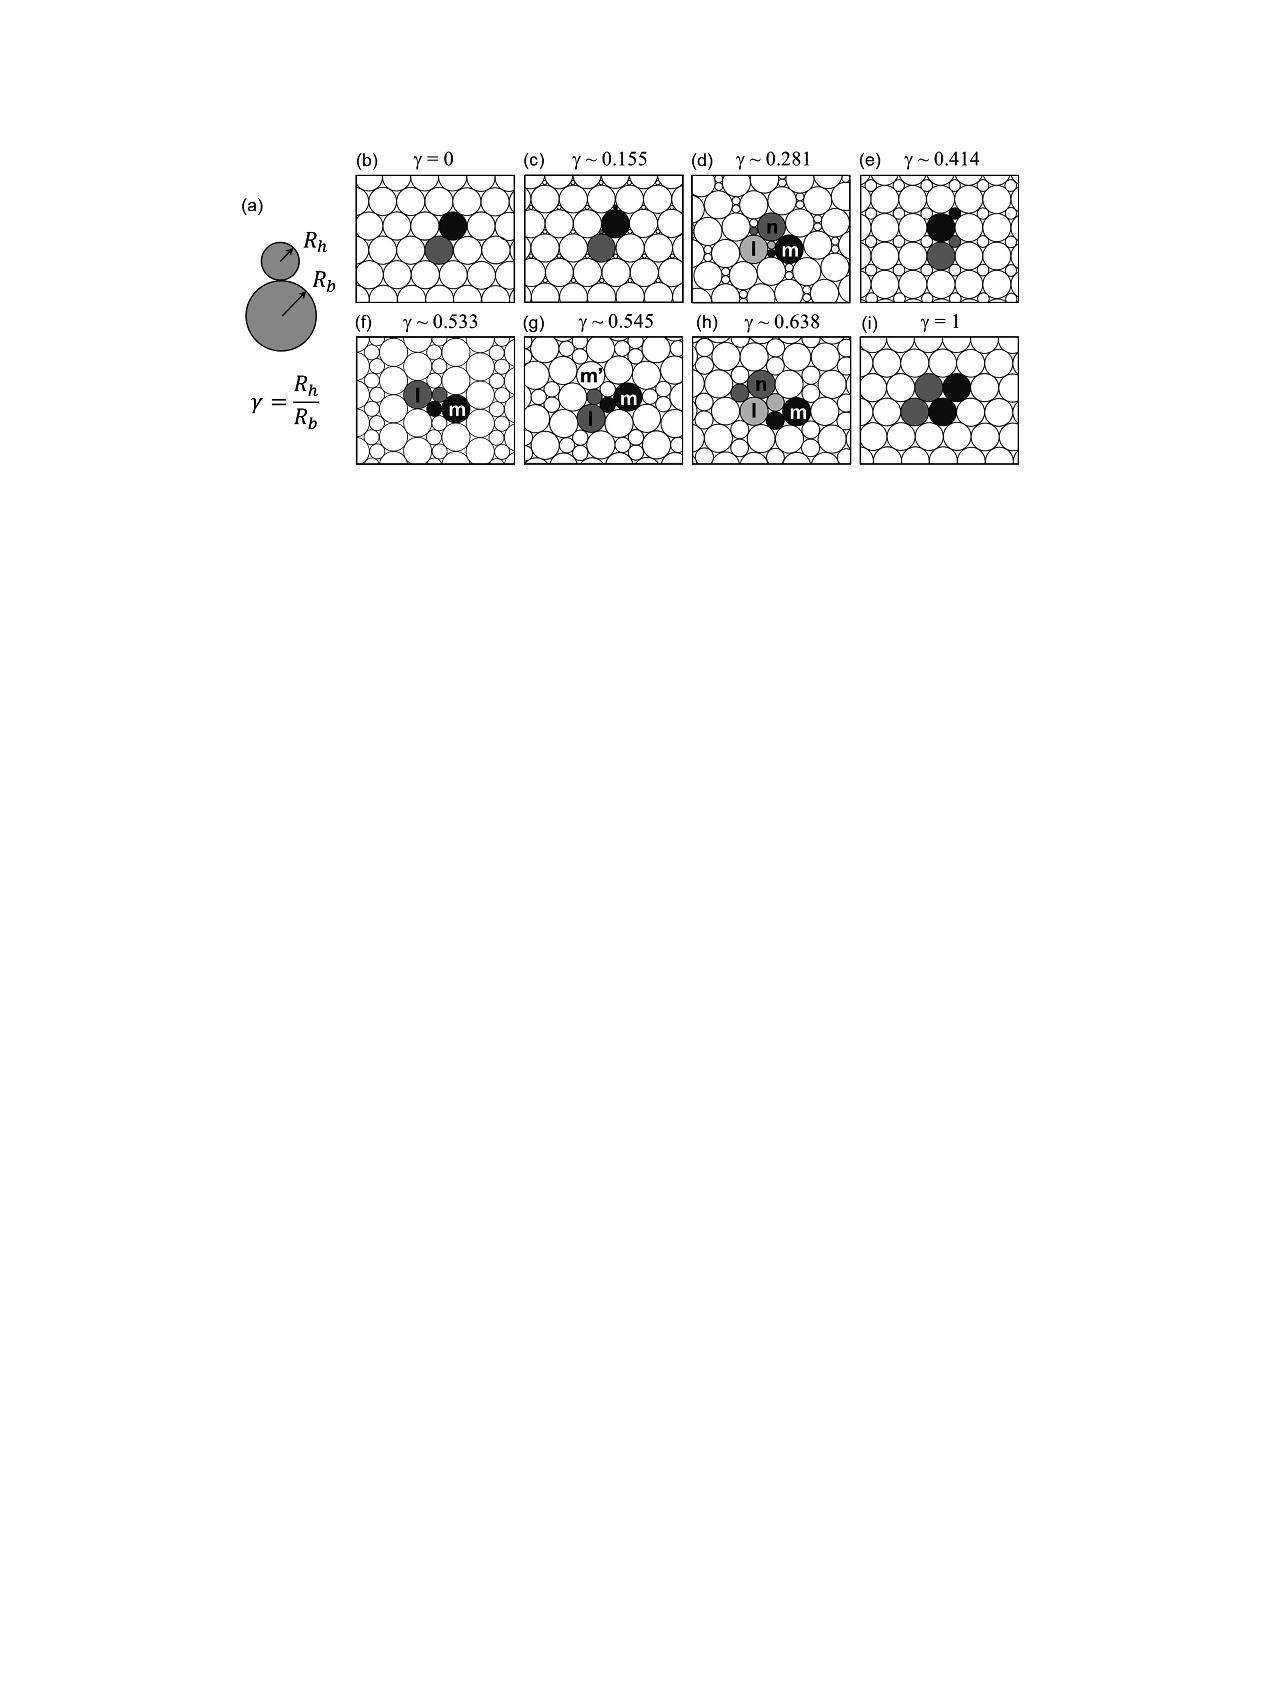
\includegraphics[width=\textwidth]{binary-packings}
    \caption[Perfect binary packings]{The eight perfect equimolar binary packings. All of these are maximums in the packing of space by snowmen crystals.}
    \source{han:13}{American Physical Society}
    \label{fig:binary-packings}
\end{figure}

For trimers the extra dimension makes a complete too computationally expensive. Instead it makes sense to focus on the remaining dimension, the angle, over a range of radii and at both $d=1$ and $d=1+r$.


\section{Packing Dimers}

The packing fraction is a concept used to asses the packing of hard shapes and it can also describe the packing of soft shapes. Taking the inherent structures after equilibration at a temperature of 3.0, the packing fraction of the Snowmen is shown in \textfigref{snowman dist high} and \textfigref{snowman radius high}. As the distance increases from $1$ to $1+r$ the packing fraction drops, this is a result of the overlap of the molecule increasing. At $d=1+r$ the two particles are touching, decreasing the distance results in overlap and a filling of the space between the molecules that was previously unoccupied. The decrease in packing fraction as a function of distance breaks down for four molecules, $d=1+0.8r, 1+r$ and $r=0.9, 1.0$. The cause of this anomaly is not immediately obvious, since our simulations are in two dimensions we can examine the configuration~\figref{snowman 0.9 1.7 frame high}. Here we can see a high degree of order in the packing, while the orientation of the bonds is distributed randomly the packing is crystalline.

\begin{figure}
    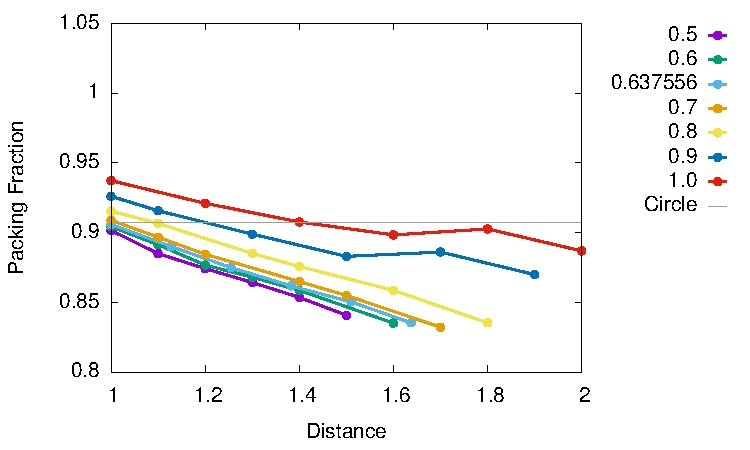
\includegraphics[width=0.5\textwidth]{dist-high}
    \caption[Packing fraction of snowmen as a function of distance ($T=3.0$)]{The packing fraction as a function of distance for the snowman molecules. For reference the optimal circle packing of 0.91 is included.}
    \label{fig:snowman dist high}
\end{figure}

\begin{figure}
    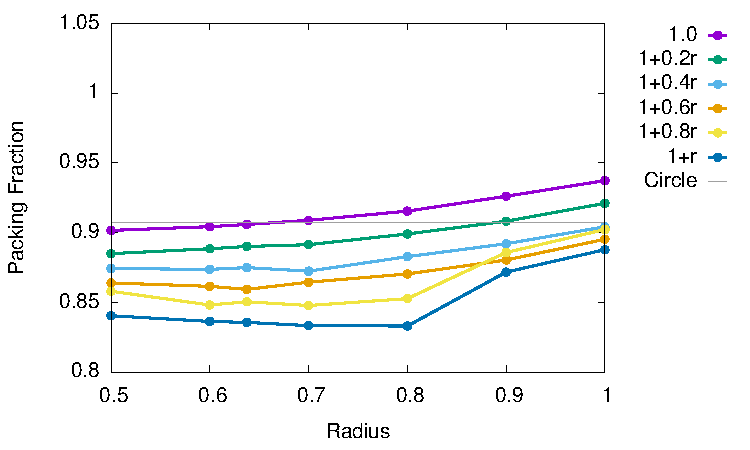
\includegraphics[width=0.5\textwidth]{radius-high}
    \caption[Packing fraction of snowmen as a function of radius ($T=3.0$)]{The packing fraction as a function of radius for the snowman molecules. For reference the optimal circle packing of 0.91 is included.}
    \label{snowman dist high}
\end{figure}

\begin{figure}
    \includegraphics[width=\textwidth]{{{Snowman-0.9-1.7-frame-high}}}
    \caption[Inherent structure of Snowman $r=0.9$ $d=1.7$]{Inherent structure of the Snowman $r=0.9$ $d=1.7$.}
    \label{fig:snowman 0.9 1.7 frame high}
\end{figure}

When an crystal structure has an orientationally ordered state and a randomly oriented state at the same energy level, it is going to form the disordered state. The extra free energy gained from the entropy of the random orientation at higher temperatures will overcome the small differences in entropy from a slightly misaligned structure. This orientational disorder is something that can be found in all the compact packings, using the compact packing of the $0.637556$ binary disc mixture.

\begin{figure}
    \includegraphics[width=\textwidth]{{{snowman-0.637556-1.637556-random}}}
    \caption{Random orientation of bonds within a compact binary packing can be randomly oriented}
    \source[\ccbysa]{dense-packing}
    \label{fig:snowman 0.637556 1.637556 random}
\end{figure}



